% Blocks 4a + 4b — prototype-similarity output + sampler chain.
% Full-width standalone. Compile:  pdflatex arch_expand_output.tex

\documentclass[tikz,border=8pt]{standalone}
\usepackage{tikz}
\usepackage{amsmath,amssymb}
\usepackage{xcolor}
\usetikzlibrary{positioning,arrows.meta,calc,fit,backgrounds,decorations.pathreplacing}

\newcommand{\bP}{\mathbf{P}}
\newcommand{\bs}{\mathbf{s}}
\newcommand{\bz}{\mathbf{z}}
\newcommand{\bipset}{\{-1,+1\}}

\definecolor{cBipolar}{HTML}{2C5282}
\definecolor{cBipolarLite}{HTML}{EBF4FF}
\definecolor{cCont}{HTML}{B7791F}
\definecolor{cContLite}{HTML}{FFF8E6}
\definecolor{cSampler}{HTML}{6B46C1}
\definecolor{cSamplerLite}{HTML}{F3EBFF}
\definecolor{cOp}{HTML}{2D3748}
\definecolor{cPanelBg}{HTML}{FAFBFC}
\definecolor{cPanelBorder}{HTML}{CBD5E0}
\definecolor{cArrow}{HTML}{1A202C}

\tikzset{
  block/.style={draw=cPanelBorder, fill=cPanelBg, thick, rounded corners=6pt,
                inner sep=8pt, minimum width=170mm},
  blockTitle/.style={font=\bfseries\normalsize, anchor=north west, inner sep=6pt},
  cellPos/.style={draw=cBipolar!50, fill=cBipolarLite, font=\small,
                  minimum width=9mm, minimum height=8mm, inner sep=0pt},
  cellNeg/.style={draw=cBipolar!50, fill=cBipolar!18, font=\small,
                  minimum width=9mm, minimum height=8mm, inner sep=0pt},
  cellCont/.style={draw=cCont!60, fill=cContLite, font=\small,
                   minimum width=13mm, minimum height=8mm, inner sep=0pt},
  cellPlain/.style={draw=black!30, fill=white, font=\small,
                    minimum width=9mm, minimum height=8mm, inner sep=0pt},
  op/.style={draw=cOp, fill=white, thick, circle, inner sep=1.4pt,
             font=\small, minimum size=7mm},
  flow/.style={-{Stealth[length=2.2mm]}, thick, draw=cArrow},
  recur/.style={-{Stealth[length=2.2mm]}, thick, draw=cCont!80!black, dashed},
  lbl/.style={font=\scriptsize\itshape, text=black!65, align=center},
  matlbl/.style={font=\scriptsize, text=cBipolar!85!black, align=center},
  idx/.style={font=\scriptsize\ttfamily, text=black!55},
}

\begin{document}
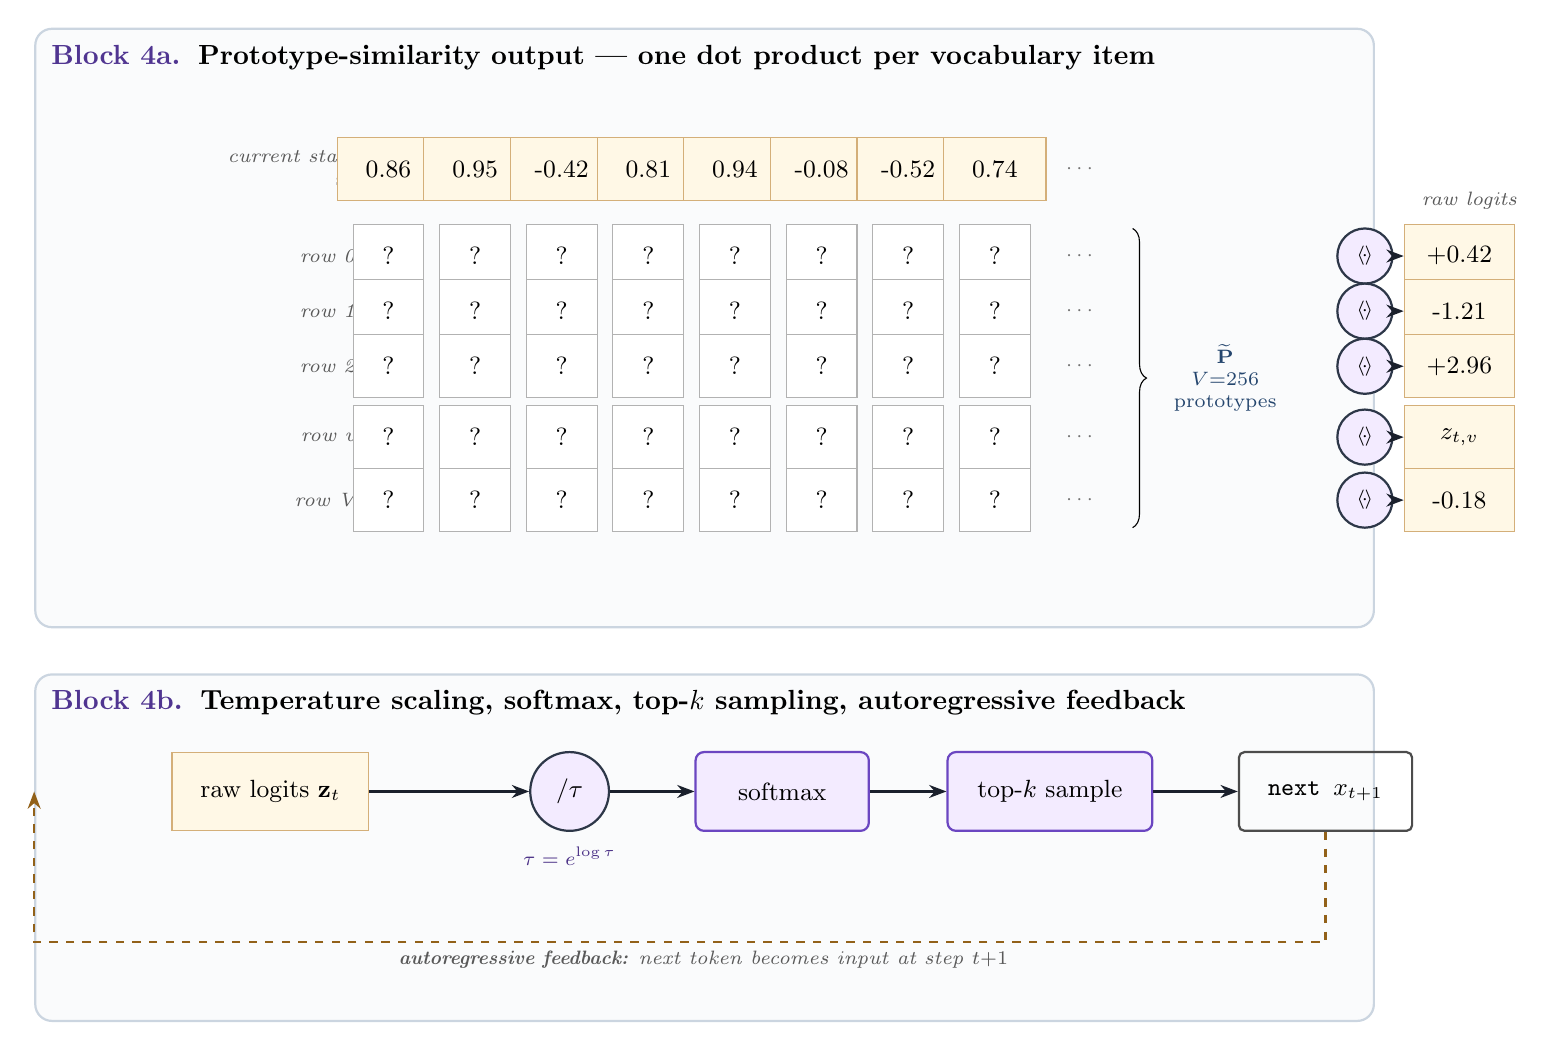
\begin{tikzpicture}

% ========== BLOCK 4a: PROTOTYPE ==========
\node[block, minimum height=76mm, anchor=north west] (B4a) at (0,0) {};
\node[blockTitle] at (B4a.north west)
  {\textcolor{cSampler!75!black}{Block 4a.}\;\;Prototype-similarity output --- one dot product per vocabulary item};

\begin{scope}[shift={(4.5,-1.8)}]
  \node[lbl, anchor=east, align=right] at (-0.3, 0)
    {current state\\$\bs_t$};
  \foreach \v [count=\i from 0] in {0.86,0.95,-0.42,0.81,0.94,-0.08,-0.52,0.74} {
    \node[cellCont] (ss\i) at (\i*1.1, 0) {\v};
  }
  \node[idx] at (8*1.1, 0) {$\cdots$};

  \foreach \row/\y/\pat in {0/-1.1/{+,+,-,-,+,+,-,-},
                            1/-1.8/{-,+,+,-,-,+,+,-},
                            2/-2.5/{+,-,+,-,+,-,+,-},
                            v/-3.4/{?,?,?,?,?,?,?,?},
                            V/-4.2/{-,-,+,+,-,+,-,+}} {
    \node[lbl, anchor=east] at (-0.3, \y) {row \row};
    \foreach \v [count=\i from 0] in \pat {
      \ifx\v+
        \node[cellPos] (p\row_\i) at (\i*1.1, \y) {$+$};
      \else\ifx\v-
        \node[cellNeg] (p\row_\i) at (\i*1.1, \y) {$-$};
      \else
        \node[cellPlain] (p\row_\i) at (\i*1.1, \y) {?};
      \fi\fi
    }
    \node[idx] at (8*1.1, \y) {$\cdots$};
  }

  \draw[decorate, decoration={brace, amplitude=5pt}]
    (8*1.1 + 0.65, -0.75) -- (8*1.1 + 0.65, -4.55);
  \node[matlbl, anchor=west] at (8*1.1 + 1.05, -2.65)
    {$\widetilde\bP$\\$V{=}256$\\prototypes};

  \foreach \row/\y/\val in {0/-1.1/{+0.42},
                            1/-1.8/{-1.21},
                            2/-2.5/{+2.96},
                            v/-3.4/{$z_{t,v}$},
                            V/-4.2/{-0.18}} {
    \node[op, fill=cSamplerLite] (dot\row) at (12.4, \y)
       {\scriptsize$\langle\!\cdot\!\rangle$};
    \node[cellCont, minimum width=14mm] (lg\row) at (13.6, \y) {\val};
    \draw[flow] (dot\row) -- (lg\row);
  }
  \node[lbl, anchor=west] at (13.0, -0.4) {raw logits};
\end{scope}

% ========== BLOCK 4b: SAMPLER ==========
\node[block, minimum height=44mm, anchor=north west] (B4b) at (0,-82mm) {};
\node[blockTitle] at (B4b.north west)
  {\textcolor{cSampler!75!black}{Block 4b.}\;\;Temperature scaling, softmax, top-$k$ sampling, autoregressive feedback};

\begin{scope}[shift={(3.0,-9.7)}]
  \node[cellCont, minimum width=25mm, minimum height=10mm]
    (rawZ) at (0, 0) {raw logits $\bz_t$};
  \node[op, fill=cSamplerLite, minimum size=10mm] (divT) at (3.8, 0) {$/\tau$};
  \node[draw=cSampler, fill=cSamplerLite, thick, rounded corners=3pt,
        minimum width=22mm, minimum height=10mm, font=\small]
        (sm) at (6.5, 0) {softmax};
  \node[draw=cSampler, fill=cSamplerLite, thick, rounded corners=3pt,
        minimum width=26mm, minimum height=10mm, font=\small]
        (tk) at (9.9, 0) {top-$k$ sample};
  \node[draw=black!70, thick, rounded corners=2pt, minimum width=22mm,
        minimum height=10mm, font=\small\ttfamily]
        (nxt) at (13.4, 0) {next $x_{t+1}$};

  \draw[flow] (rawZ) -- (divT);
  \draw[flow] (divT) -- (sm);
  \draw[flow] (sm)   -- (tk);
  \draw[flow] (tk)   -- (nxt);

  \node[lbl, below=2pt of divT, text=cSampler!70!black]
     {$\tau = e^{\log\tau}$};

  \draw[recur] (nxt.south) -- ++(0,-1.4) -| (-3.0, 0);
  \node[lbl, align=center, anchor=north] at (5.5, -1.9)
    {\textbf{autoregressive feedback:} next token becomes input at step $t{+}1$};
\end{scope}

\end{tikzpicture}
\end{document}
